\subsection{Within-Database Performance Evaluation}

\subsubsection{Contactless Finger Knuckle Image Database (Version 3.0)}

The finger knuckle database \cite{fingerknuckledbv3.0} can offer contactless finger knuckle of 221 subjects, but only 104 subjects have second session samples. For each session, each subject can offer 6 samples. It is worth mentioning that the finger knuckle sample provided by this database is more challenging and closer to real world scenarios, because the finger knuckle will bend from 0 to 90 degree result in crease deformation.

\textbf{One-Session Protocol}

As for the one-session protocol, I firstly fine-tuned models on the second session 104 subjects dataset, totally $104 * 6 = 624$ images as the testing set. Then use the first session 221 subjects as the testing set result in $221*6=1326$ genuine matching scores and $221*220*6=291720$ imposter matching scores. From the Figure \ref{fkv3-one-session}, we can easily find the RFNet is the best model not only on the ROC but also on the CMC. In terms of the baseline model RFNet, our loss function TRTL can improve the matching accuracy when compare to the STTL loss function. Although the finger knuckle of the database with deformation while bend from 0 to 90 degree, the EER of the RFNet-TRTL can arrive at $2.21\%$. As for the rest model, EfficientNetV2-S model performance is better than FKNet and DeConvRFNet.

\begin{figure}[ht!]
	\centering
	\begin{subfigure}[b]{0.45\linewidth}
		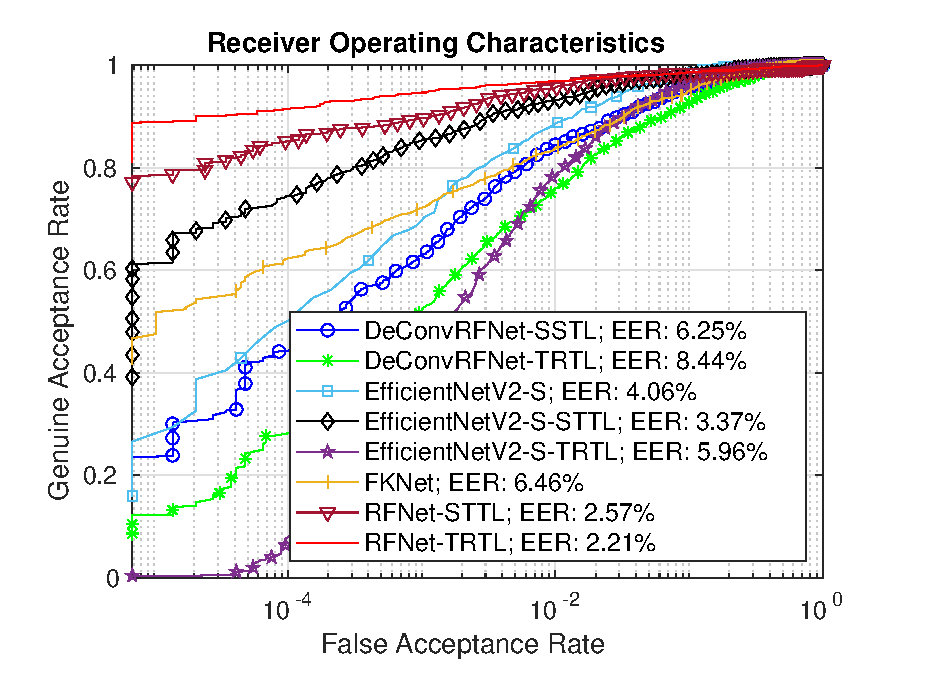
\includegraphics[width=\linewidth]{Figures/fkv3-roc_compare_new.eps}
		\caption{}
	\end{subfigure}
	\begin{subfigure}[b]{0.45\linewidth}
		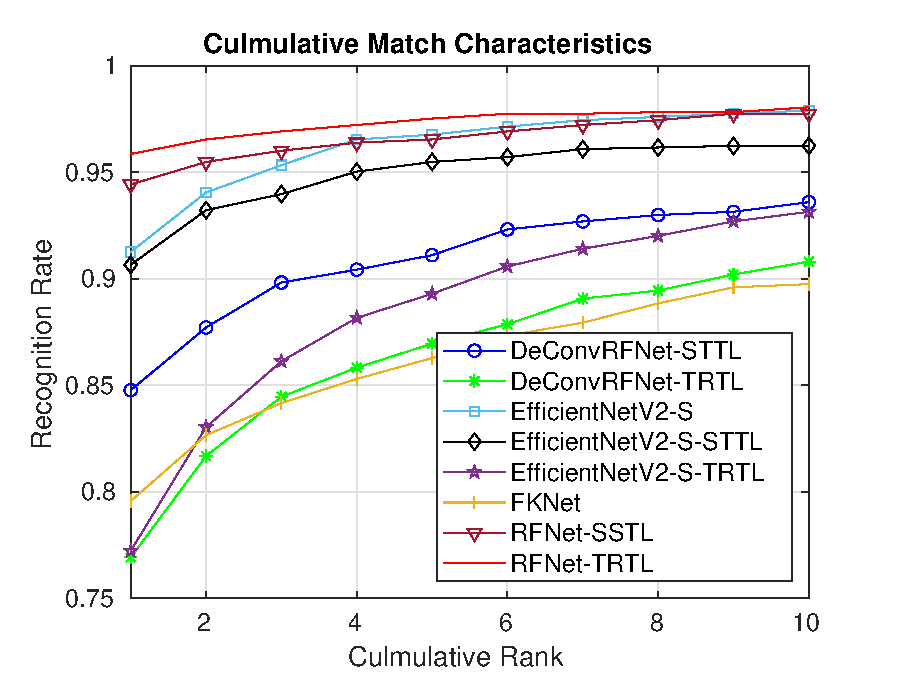
\includegraphics[width=\linewidth]{Figures/fkv3-cmc_compare_new.eps}
		\caption{}
	\end{subfigure}
	\caption{Comparative ROC (a) and corresponding CMC (b) for one-session on the contactless finger knuckle image database \cite{fingerknuckledbv3.0}.}
	\label{fkv3-one-session}
\end{figure}

\textbf{Two-Session Protocol}

We fine-tune models on the first session subjects who don't provide second session samples, and use two-session protocol to evaluate my model performance on the first session subjects who can offer two-session data. In totally, it will generate $104*6=624$ genuine scores, and $104*103*6$ imposter scores. Just like said before, the FKNet and EfficientNetV2-S are classification networks, we use output feature vector to calculate MSE as the matching score. Because the degree of deformation vary on the two-session data, the verification and identification scenarios is more complexity than one-session protocol. Due to these factors, the accuracy on the two-session protocol is much lower than the one-session protocol. However, the RFNet is still the best model, even its EER is half of the EER of other models. Meanwhile, our TRTL loss function still work better than the STTL loss function, with $16.65\%$ and $18.35\%$ respectively. From the ROC and CMC Figure \ref{fkv3-two-session}, we can also get that the STTL and TRTL triplet loss function are better than classification task, because the FKNet and EfficientNetV2-S have the lowest accuracy.

\begin{figure}[ht!]
    \centering
	\begin{subfigure}[b]{0.45\linewidth}
		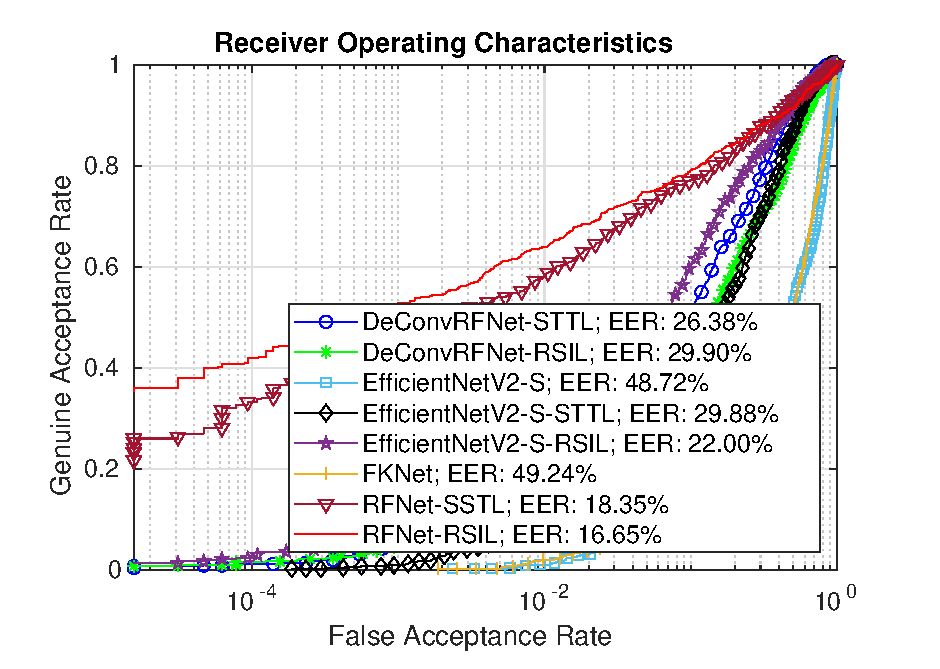
\includegraphics[width=\linewidth]{Figures/two-fkv3roc_compare_new.eps}
		\caption{}
	\end{subfigure}
	\begin{subfigure}[b]{0.45\linewidth}
		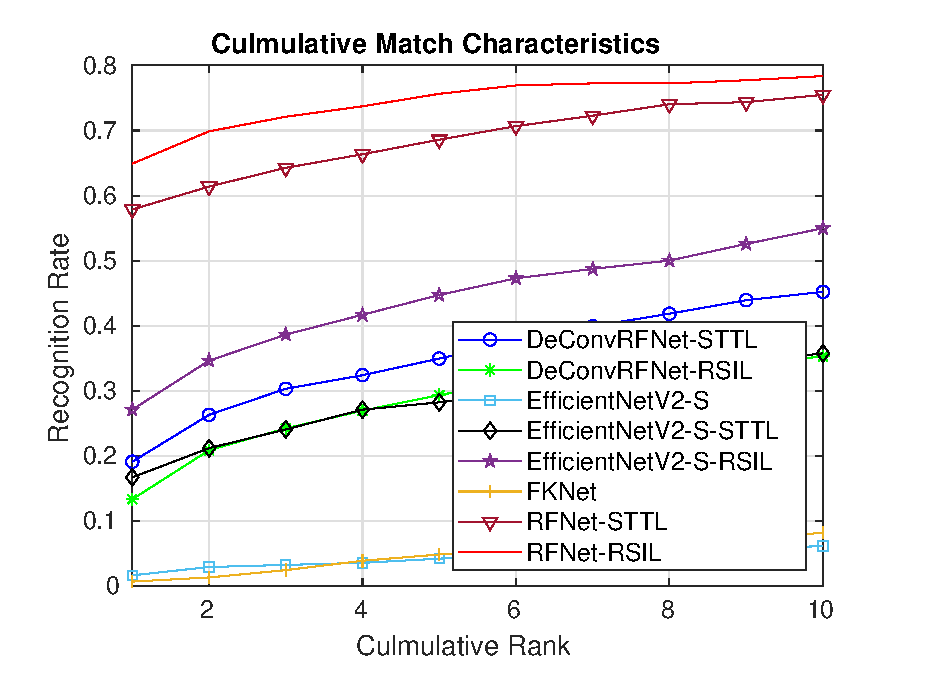
\includegraphics[width=\linewidth]{Figures/two-fkv3cmc_compare_new.eps}
		\caption{}
	\end{subfigure}
	\caption{Comparative ROC (a) and corresponding CMC (b) for two-session on the contactless finger knuckle image database \cite{fingerknuckledbv3.0}.}
	\label{fkv3-two-session}
\end{figure}


\subsubsection{Index Finger Knuckle of Contactless Hand Dorsal Image Database}

\begin{figure}[ht!]
	\centering
	\begin{subfigure}[b]{0.45\linewidth}
		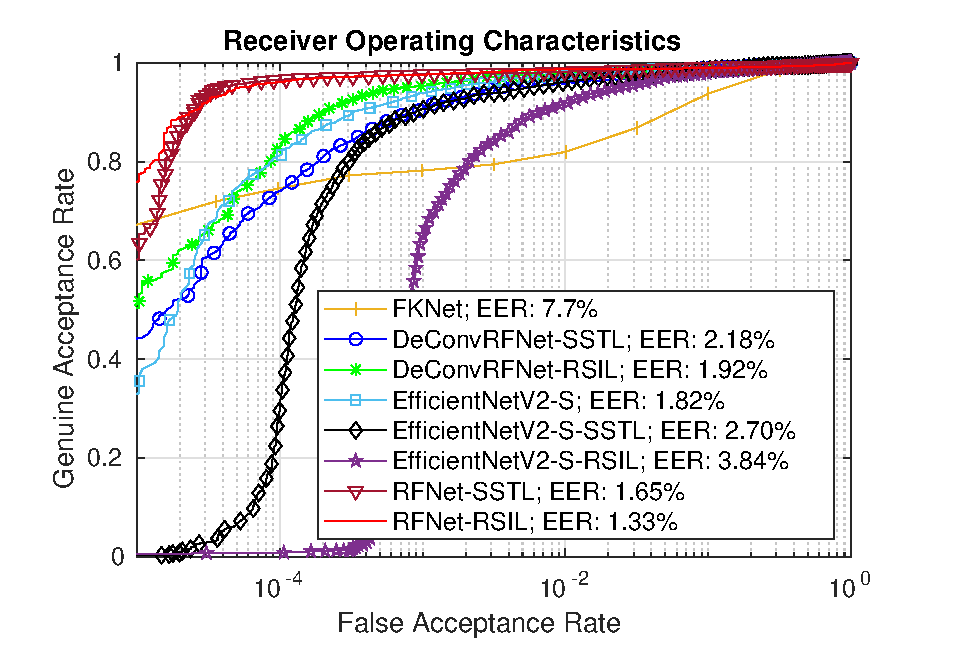
\includegraphics[width=\linewidth]{Figures/hd-roc_compare_new.eps}
		\caption{}
	\end{subfigure}
	\begin{subfigure}[b]{0.45\linewidth}
		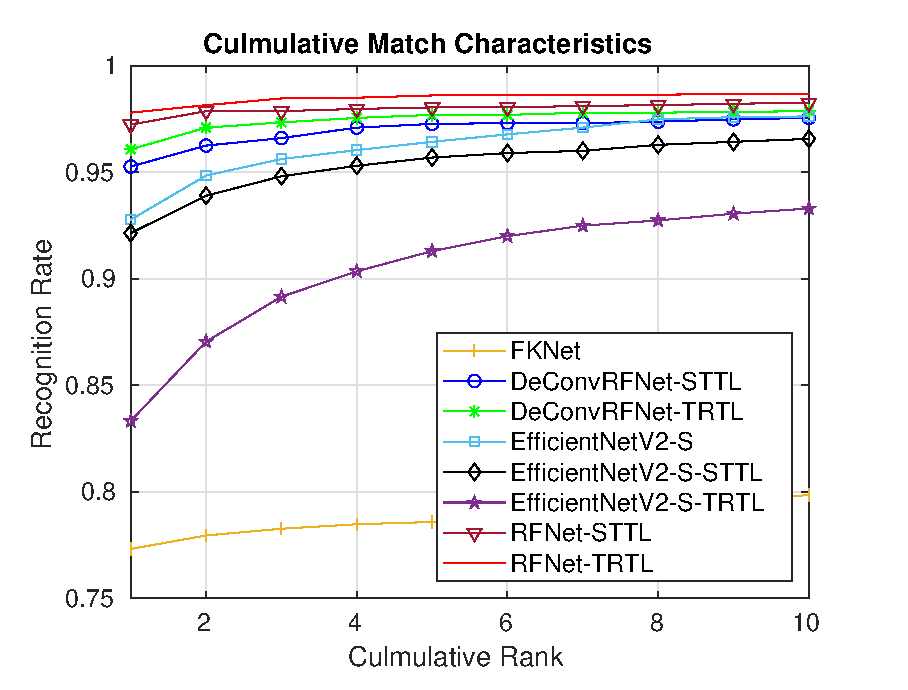
\includegraphics[width=\linewidth]{Figures/hd-cmc_compare_new.eps}
		\caption{}
	\end{subfigure}
	\caption{Comparative ROC (a) and corresponding CMC (b) for one-session on the contactless hand dorsal image database \cite{ContactlessHnadDorsaldb}.}
	\label{hd-one-session}
\end{figure}

As for the experiment, the dataset \cite{ContactlessHnadDorsaldb} totally contains 712 subjects. And we fine-tuned our models on the first sample of each subject, and then use the rest four sample as the testing dataset. The protocol follow the same protocol of the FKNet \cite{cheng2020deep} 

At the testing process, it has $712*4=2848$ genuine matching scores, and has $712*711*4=2024928$ imposter matching scores. The performance of RFN-128-WRS and RFN-128-WS is similar, but the RFN-128-WS is slightly better than RFN-128-WRS depend on the EER value. And we can get an information that the RFNet is better than the rest network in the ROC figure, including the FKNet.


\subsubsection{2D Samples of 3D Finger Knuckle Database}

First experiment on the database is to use the one session 190 subjects image to fine-tune models and then to test on the another session 190 subjects. It has $190*6$ genuine matching scores and $190*189*6$ imposter matching scores. From the result, we can see that these RFN-128-WRS, RFN-128-WS, EfficientNetV2 can get very high matching accuracy. Meanwhile, the RFNet-TRTL has the minimal EER value among these models. As for the FKNet performance, it gets a very bad result on the 2D images of 3D finger knuckle. I think I have fully trained the FKNet. Maybe the model is overfitting on the training dataset.

\begin{figure}[H]
	\centering
	\begin{subfigure}[b]{0.45\linewidth}
		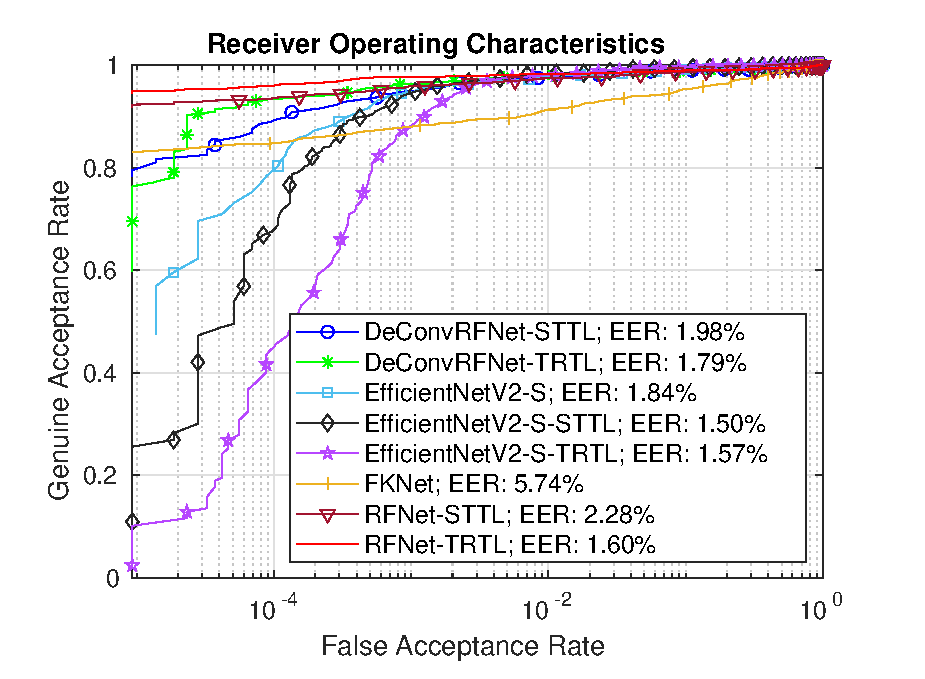
\includegraphics[width=\linewidth]{Figures/2dof3d-roc_compare_new.eps}
	\end{subfigure}
	\begin{subfigure}[b]{0.45\linewidth}
		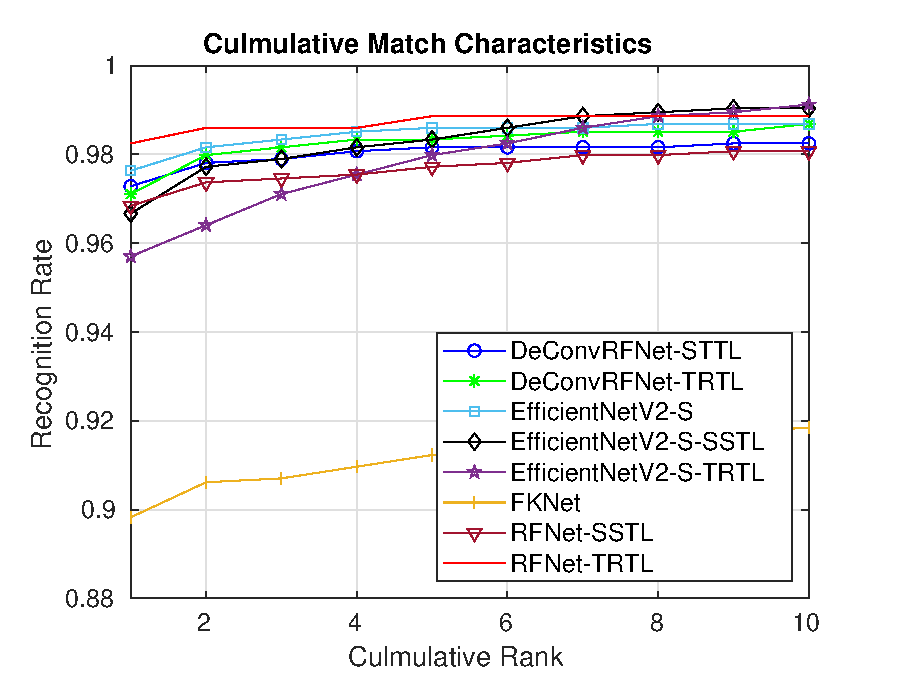
\includegraphics[width=\linewidth]{Figures/2dof3d-cmc_compare_new.eps}
	\end{subfigure}
\end{figure}


And then use the two session protocol. I use the rest samples of session1, and it has 191-228 subjects. In this kind of situation, the training dataset is too small. The two session protocol will test on the 190 subjects, these subjects can offer two session samples. Due to the training set is too small, so the matching performance is not very good. As for the FKNet, it cannot fit on two session protocol due to classification task.
